\chapter{Crypto.Asymmetric.DSA}
In this generic package the implementation of DSA (Digital Signature
Algorithm) is provided. It was proposed by the National Institute of
Standards and Technology (NIST) in August 1991 for use in their
Digital Signature Standard (DSS), specified in \cite{DSA-FIPS}.

With DSA man can produce digital signatures and verify their
authenticity. To sign a message you need a public key and a private
key. The private key is used during the signature process and the
public key is used during the verification process. In the signature
process what is being signed is not the message, but the SHA-1 hash
value (Chapter \ref{Hash}) of the message. Who doesn't know the
private key can't produce a valid (verifiable) signature, but who
knows the public key can be able to verify the correctness of a
signature by running the verification process.
\subsubsection*{Generic Part}
\begin{lstlisting}{}
  generic
    Size : Positive;
\end{lstlisting}
\textbf{Exception:} If Size $\neq 512+64*I$\,, where
$I\in\{0,\cdots,8\}$:\quad \texttt{Constraint\_Size\_Error}.\\
\section{API}
Figure \ref{StructureDSA} shows the workflow of DSA.
\begin{figure}[h]
\centering
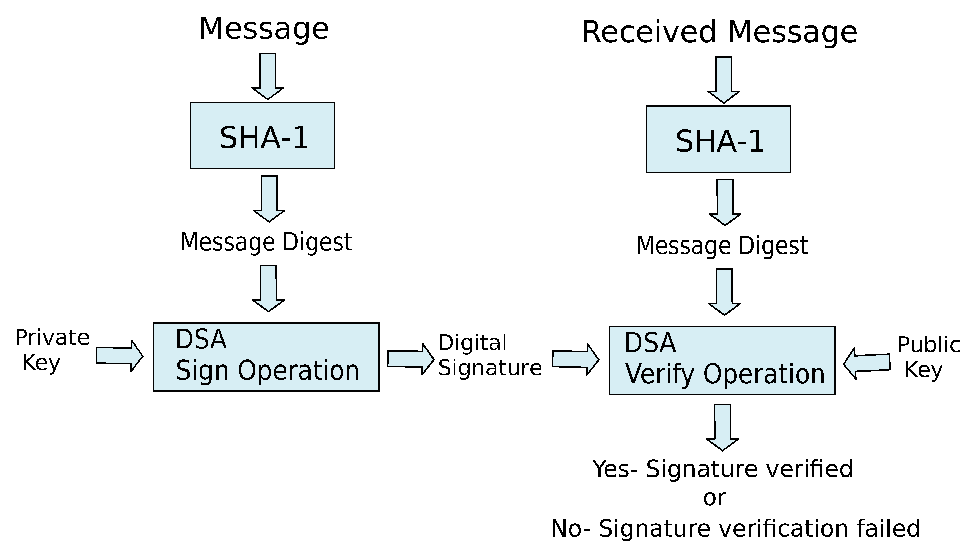
\includegraphics[scale=0.7]{./images/DSA_En_De}
\caption{Workflow of the DSA algorithm. Adapted from
  \cite{DSA-FIPS}.}\label{StructureDSA}
\end{figure}
\subsubsection*{Types}
\begin{lstlisting}{}
  subtype DSA_Number is Bytes(0..Size/8-1);
  type Public_Key_DSA  is private;
  type Private_Key_DSA is private;
  type Signature_DSA   is private;
\end{lstlisting}
The \texttt{DSA\_Number} is a byte array which interprets a
number. Its first element ($'First$) corresponds the most significant
byte and the last element ($'Last$) corresponds the least significant
byte of the number.\\ As required in DSA, each key has four
parameters:
\begin{lstlisting}{}
  type DSA_KEY is record
      P : Big_Unsigned;
      Q : Big_Unsigned;
      G : Big_Unsigned;
      K : Big_Unsigned;
  end record;
  type Public_Key_DSA is new DSA_KEY;
  type Private_Key_DSA is new DSA_KEY;
\end{lstlisting}

\subsubsection*{Procedures}
\begin{lstlisting}{}
  procedure Gen_Key(Public_Key  : out Public_Key_DSA;
                    Private_Key : out Private_Key_DSA);
\end{lstlisting}
This procedure generates a pair of keys, which are a public key
(\texttt{Public\_Key}) and a private key
(\texttt{Private\_Key}).

\noindent\textbf{Exception:} If the value $P$ of the
public key is less than 3:\quad\texttt{Constraint\_Error}.


\hhline
\begin{lstlisting}{}
  procedure Sign(Private_Key : in  Private_Key_DSA;
                 SHA1_Hash   : in  W_Block160;
                 Signature   : out Signature_DSA);
\end{lstlisting}
This procedure signs the SHA-1 hash value (\texttt{SHA1\_Hash}) of a
message with a private key (\texttt{Private\_Key}).

\hhline
\begin{lstlisting}{}
  function Verify(Public_Key  : Public_Key_DSA;
                  SHA1_Hash   : W_Block160;
                  Signature   : Signature_DSA) return Boolean;
\end{lstlisting}
This function returns true if the signature can be verified with the
public key (\texttt{Public\_Key}) to be a valid signature of the SHA-1
hash value (\texttt{SHA1\_Hash}). If not, then false is
returned.\\

With the public key only the signature created from the
related private key can be verified. If the two keys don't match
together, then the function returns false.\\

But if Bob uses the
identity card of Alice, then we can't make identification of Bob with
the card, although the identity card of Alice is valid.

\hhline
\begin{lstlisting}{}
  procedure Sign_File(Filename    : in  String;
                      Private_Key : in  Private_Key_DSA;
                      Signature   : out Signature_DSA);
\end{lstlisting}
With this procedure we can sign a file (\texttt{Filename}) with the
private key (\texttt{Private\_Key}).\\

\noindent\textbf{Exception:}\\
 If the \texttt{Private\_Key} is not initialized:\quad
 \texttt{Invalid\_Private\_Key\_Error}.

\begin{lstlisting}{}
  function Verify_File(Filename   : String;
                       Public_Key : Public_Key_DSA;
                       Signature  : Signature_DSA)
                       return Boolean;
\end{lstlisting}
This function returns true if the signature can be verified with the
public key (\texttt{Public\_Key}) to be a valid signature of the file
(\texttt{Filename}). If not, false is returned.\\

With the public key only the signature created from the related
private key can be verified. If the two keys don't match together,
then the function returns false.\\


\noindent\textbf{Exception:}
If the \texttt{Public\_Key} is not initialized :\quad \texttt{Invalid\_Public\_Key\_Error}.

\hhline
\begin{lstlisting}{}
  function Verify_Key_Pair(Private_Key : Private_Key_DSA;
                           Public_Key  : Public_Key_DSA) 
                           return Boolean;
\end{lstlisting}
This function returns true if the two keys \texttt{Private\_Key} and
\texttt{Public\_Key} match to each other, that is, they are a pair, if
not, then false is returned.

\hhline
\begin{lstlisting}{}
  procedure Get_Public_Key(Public_Key : in Public_Key_DSA;
                           P          : out DSA_Number;
                           Q          : out DSA_Number;
                           G          : out DSA_Number;
                           Y          : out DSA_Number);
\end{lstlisting}
This procedure decomposes a public key (\texttt{Public\_Key}) into
four components:
\begin{itemize}
\item One size-bit prime number $P$
\item One 160 bit prime number $Q$
\item One generator $G$ which $G=H^{(P-1)/Q}\mod P,\quad 1<H<P-1$
\item The real public key $Y$
\end{itemize}
With the four components the public key can be reconstructed later.

\hhline
\begin{lstlisting}{}
  procedure Get_Private_Key(Private_Key : in Private_Key_DSA;
                            P           : out DSA_Number;
                            Q           : out DSA_Number;
                            G           : out DSA_Number;
                            X           : out DSA_Number);
\end{lstlisting}
The private key \texttt{Private\_Key} is decomposed into four components:
\begin{itemize}
\item One size-bit prime number $P$
\item One 160 bit prime number $Q$
\item One generator $G$ which $G=H^{(P-1)/Q}\mod P,\quad 1<H<P-1$
\item The real private key $X$
\end{itemize}
With the four components the private key can be reconstructed later.

\hhline
\begin{lstlisting}{}
  procedure Set_Public_Key(P          : in DSA_Number;
                           Q          : in DSA_Number;
                           G          : in DSA_Number;
                           Y          : in DSA_Number;
                           Public_Key : out Public_Key_DSA);
\end{lstlisting}
During this procedure a public key can be (re-)constructed. The
following values are required:
\begin{itemize}
\item One size-bit prime number $P$
\item One 160 bit prime number $Q$
\item One generator $G$ which is a subgroup of $Z^*_P$ with order $Q$
\item The real public key $Y$
\end{itemize}
\textbf{Exception:}\\
 If any of the following conditions is met, then the
 \texttt{Invalid\_Public\_Key\_Error} is raised:
\begin{enumerate}
\item the length of $P$ is not equal the \texttt{Size}\,,
\item the length of $Q$ is not 160 bits\,,
\item the term $G$ is not in the range: $1<G<P$\,,
\item the term $Y$ is equal zero\,.
\end{enumerate}

\hhline
\begin{lstlisting}{}
  procedure Set_Private_Key(P           : in DSA_Number;
                            Q           : in DSA_Number;
                            G           : in DSA_Number;
                            X           : in DSA_Number;
                            Private_Key : out Private_Key_DSA);
\end{lstlisting}
A private key can be (re-)constructed. The following values are required:
\begin{itemize}
\item One size-bit prime number $P$
\item One 160-bit prime number $Q$
\item One generator $G$ which is a subgroup of $Z^*_P$ with order $Q$
\item The real private key $X$
\end{itemize}
\noindent\textbf{Exception:}\\ 
If any of the following conditions is met, then the
\texttt{Invalid\_Private\_Key\_Error} is raised:
\begin{enumerate}
\item the length of $P$ is not equal the \texttt{Size}\,,
\item the length of $Q$ is not 160 bits\,,
\item the term $G$ is not in the range: $1<G<P$\,,
\item the term $X$ is equal zero\,.
\end{enumerate}

\subsubsection*{Example}
\begin{lstlisting}{}
  with Ada.Text_IO;
  with Crypto.Types.Big_Numbers;
  with Crypto.Asymmetric.DSA;
  use Ada.Text_IO;
  procedure Example_DSA is
    package DSA is new Crypto.Asymmetric.DSA(512);
    use DSA;
    Public_Key : Public_Key_DSA;
    Private_Key : Private_Key_DSA;
    Signature : Signature_DSA;
  begin
    -- Key Generation
    Gen_Key(Public_Key, Private_Key);
    Sign_File("Example_DSA.adb", Private_Key, Signature);
    -- Verification
    if Verify_File("Example_DSA.adb", Public_Key, Signature) then
        Put_Line("OK");
    else
        Put_Line("Error");
    end if;
  end Example_DSA;
\end{lstlisting}
